%\documentclass{article}
%\usepackage{paralist} 
%\usepackage{graphicx}
%\begin{document}


\section{Security Lab Generator}
Another very important issue for research in security analytics and network security areas is providing a test network environment. To answer on the question how to automatize a process of providing a potentially vulnerable test network environments, on the past semester I devoted some time on learning and deploying the project called Security Lab Generator. Security Lab Generator (SLG) is the research project that is aimed to configure, deploy, monitor and analyze the network environments regarding security issues. The report contains an overview of the project, an overview of third-party components used in the SLG, ideas about use cases and proposals how SLG could be used for solving the issue.

\subsection{Overview}

To review the SLG project, firstly we define some definitions that will be used in this section of the report. 

\begin{compactitem}
\item Scenario - a description of the computer network. 
\item Attack graph - another view of the scenario that describes a possible attack graph for the certain network environment regarding on the location of the attacker and the hacking target.   
\item Experiment - provision resources of the scenario. Creating a network with all needed hosts and software according to the scenario.
\item Provision server - a server for running virtual machines on it. In the current case the provision server  is VirtualBox.
\end{compactitem}

The SLG project uses additional projects such as Oryx for prototyping the network environment, MulVAL for analyzing the network environment by creating attack graphs and VirtualBox for running virtual machines. SLG is written written on the java programming language with the grail framework. SLG uses the Tomcat server and the MySql database. The Oryx uses some additional components such as the PostgreSQL database and the plpython library. The MulVAL is a logic-based enterprise network security analyzer. It is used for creating an attack graph based on the prototyped scenario. The attack graph can be represented as an image with relations, as well as an XML file. The MulVAL requires additional modules such as XSB - logic programming and deductive database system and GraphViz – graph visualization software. 

The important parts of SLG are image pool and program pool components. The image pool is the container of prepared images of operations systems which can be used for deploying virtual machines. The program pool is the container of software programs that can be used for installing on virtual machines. Any new images and programs can be added to the pools.

The SLG uses the Oryx application for prototyping the network. You can see the user interface of SLG with the open Oryx editor on Figure 4. The result of prototyping can be exported as json or xml format, which describes the network scenario. The SLG xml can be converted to the input xml suitable for use in MulVAL. 

After prototyping the network, specifying each nodes and viewing the attack graph you can run the experiment. The process of running the experiment includes the creation of virtual machines with operating systems, the installation of software applications, the configuration of the network. After completion of the experiment, all resources will be installed and configured on VirtualBox. The SLG provides capability to connect to each virtual machine from the web interfaces. 

\begin{figure}[ht!]
\centering
%[width=90mm]
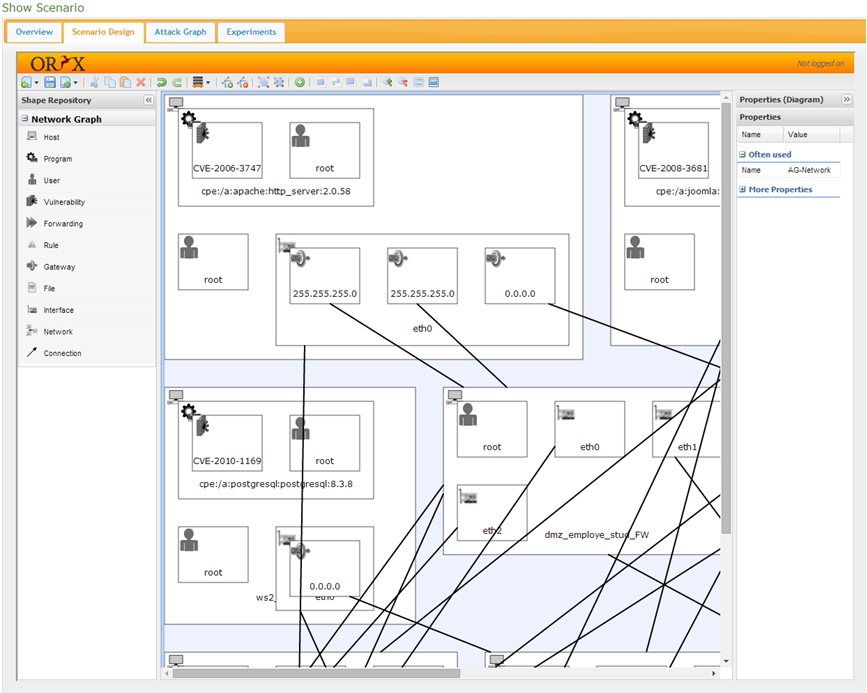
\includegraphics[width=\textwidth]{slg.png}
\caption{SLG}
\label{overflow}
\end{figure} 
SLG can be used in multiple use cases, but the main goal is to provide the platform for teaching and study of network security issues and the creation testbeds for research in security analytics and network security areas. For example, it can be used for Capture The Flag (CTF) seminars.


As the platform for teaching SLG could be used for Capture The Flag (CTF) seminars. The idea of the seminar is that the tutor deploys a potentially vulnerable network with vulnerable applications. Students, in turn, are trying to gain access to the network and virtual machines using found vulnerabilities to find flags. The flag is some label or code. The SLG should provide capability not only to deploy the network environment, but also to monitor user activities, find out compromised machines, make a report on ways of hacking the system. But these features do not implemented yet. 
  
  
In the this section we just learned Security Lab Generator. On the next section we will introduce OpenStack technologies and the proposal of migrating SLG on the Cloud.
 %"4.4 Security Lab Generator based on OpenStack". 


 

%The current state of the project does not allow to use it for real seminar. SLG requires %implementation of some necessary features. 



\subsection{OpenStack at HPI}
OpenStack is open source Infrastructure as a Service that provides capability to run any complex network environments. To learn OpenStack and learn how OpenStack could be used as a basement for SLG the infrastructure was deployed at HPI servers with installed ESXi. The infrastructure includes services: Identity (Keystone), Compute (Nova), Image service (Glance), Networking (Neutron), Block Storage (Cinder), Object Storage (Swift), Dashboard (Horizon), Orchestration (Heat), Telemetry (Ceilometer). In the brackets are code names of services. On the Figure 5 you can see all VMs that are used for deploying OpenStack services. Theoretical, all services could be deployed on one VM and even there is a tool for that called DevStack\footnote{DevStack. http://devstack.org.}. But it is not option for learning or providing the basement for SLG. The Icehouse version of OpenStack and Ubuntu operation system were used for deploying OpenStack.  

The Figure 6 shows the relations between services. The Figure 7 shows the three-node architecture and which services and components nodes contain. The three-node  architecture uses three networks. The external interface is the interface that has access to the Internet. In our case is the network of ESXi server. The management interface is the interface of the network where OpenStack nodes are located. And the instance tunnels network is the network inside which all VMs with their network will be created. 

\begin{figure}[ht!]
\centering
%[width=90mm]
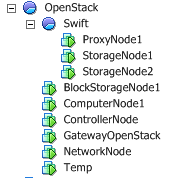
\includegraphics{openstack_tree.png}
\caption{OpenStack Nodes}
\label{overflow}
\end{figure}


\begin{figure}[ht!]
\centering
%[width=90mm]
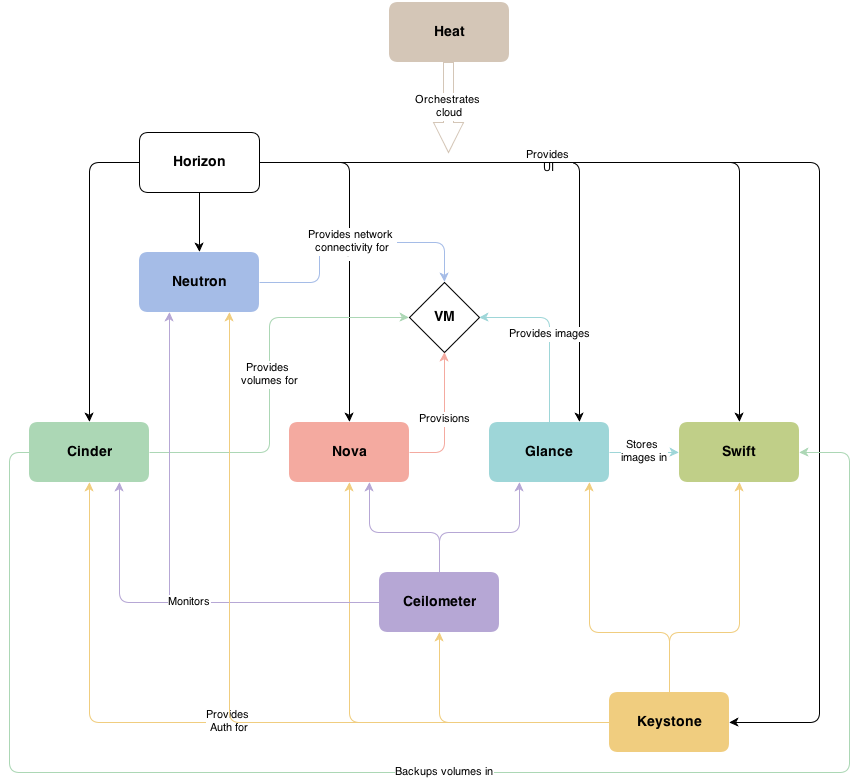
\includegraphics[width=\textwidth]{openstack_conceptual_architecture.png}
\caption{OpenStack conceptual architecture}
\label{overflow}
\end{figure}


\begin{figure}[ht!]
\centering
%[width=90mm]
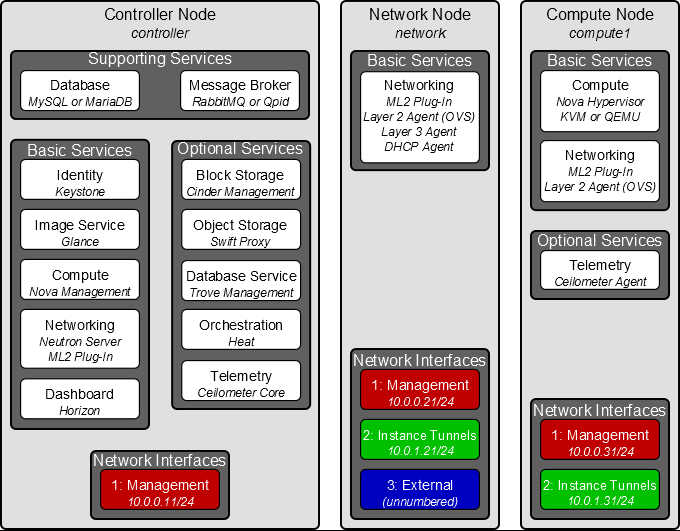
\includegraphics[width=\textwidth]{openstack_architecture.png}
\caption{OpenStack architecture}
\label{overflow}
\end{figure}

The sections just cover basic information about OpenStack. To learn more please visit official web site [5]. On the web site you can find all needed information about OpenStack, each service, installation documentation and other relevant information. 


\subsection{Security Lab Generator based on OpenStack}
The idea of Security Lab based on OpenStack (CloudSLG) is migrating the current SLG project on the cloud. It will allow to use wide functionality of IaaS in SLG interests. It means that we will not need care about how to run, configure the network, how to connect to running instances. It will allow to concentrate in solving more research questions such as analyzing user activities, finding user attack graphs, reporting analytic statistics. To migrate SLG on the cloud some challenges must be solved. The first challenge is how to convert describing network scenario xml (SLG XML) into the CloudFormation language which is used in OpenStack as well as in Amazon Web Service for running a network stack. The other challenge is how to provide the automatization of creating a specific image with vulnerable software applications.   



%\end{document} 